\subsection{Neural Tangent Kernel}\label{sec:kernels}
\textbf{Neural Tangent Kernel in `path-view':} In what follows, let $(x_s,y_s)_{s=1}^n\in\R^{d_{in}}\times\R$ be the dataset. The \emph{neural path feature} (NPF) matrix is given by $\Phi=(\phi_{x_s,\Theta},s\in[n])\in\R^{P\times n}$. The \emph{neural tangent feature} (NTF) matrix, denoted by $\Psi_{\Theta}$ is a $d_{net}\times n$ matrix, whose entries are given by $\Psi(\theta,s)=\partial_{\theta} \hat{y}_{\Theta}(x_s),\theta\in\Theta, s\in[n]$\footnote{Here $\partial_{\theta}(\cdot)$ stands for $\frac{\partial (\cdot)}{\partial \theta}$}. The \emph{neural tangent kernel} (NTK) matrix is given by $K_{\Theta}=\Psi_{\Theta}^\top\Psi_{\Theta}$. Now, thanks to the `path-view', we can further decompose the NTF and NTK by defining $d_{net}\times n$ matrices $\Psi^v_t$, and $\Psi^{\phi}_t$, whose entries are given by $\Psi^v_t(\theta,s)=\ip{\phi_{x_s,\Theta},\partial_{\theta}v_{\Theta}}$, and  $\Psi^{\phi}_t(\theta,s)=\ip{\partial_{\theta}\phi_{x_s,\Theta}, v_{\Theta}}$. Now, we have the following NTK decomposition (for a soft-ReLU DNN):
\begin{align}
K_{\Theta}=K^v_{\Theta}+K^{\phi}_{\Theta}+(\Psi^v_\Theta)^\top \Psi^{\phi}_{\Theta} +(\Psi^{\phi}_\Theta)^\top \Psi^{v}_{\Theta},\,\text{where},
\end{align}
$\bullet$ $K^v_{\Theta}$ is the NTK of path values and describes the dynamics of optimisation due to the value gradient, which, for a given input example, tunes the weights in the active sub-networks. As the GD trains the DNN, the NPFs keep evolving, and say at time $t$, we have the NPFs to be given by the matrix $\Phi_{\Theta_t}$. We let $\nabla_{\Theta}v_{\Theta}$ to be the $P\times d_{net}$ matrix consisting of the derivative of the NPVs with respect to the weights of the network, whose entries are given by $\nabla_{\Theta}v_{\Theta}(p,\theta)=\partial_{\theta}v_{\Theta}(p)$. We now expand $K^v_{\Theta}$:
\begin{align}
K^{v}_{\Theta_t}=\Phi^\top_{\Theta_t}(\nabla_{\Theta} v_{\Theta_t})(\nabla_{\Theta} v_{\Theta_t})^\top \Phi_{\Theta_t}
\end{align}
$\bullet$ $K^{\phi}_{\Theta}$ is the NTK of the features, and describes the dynamics of feature learning due to the flow of the feature gradients, which, for each input example decides, which of the sensitive yet inactive paths should become active, and which of the sensitive yet active paths should become inactive. The NTK of features can be expanded as $K^{\phi}_{\Theta}=\sum_{\theta \in \Theta}\partial_{\theta} \Phi^\top_{\theta}v_{\Theta}v^\top_{\Theta}\partial_{\theta}\Phi_{\Theta}$.\\ 
$\bullet$ $(\Psi^v_\Theta)^\top \Psi^{\phi}_{\Theta} +(\Psi^{\phi}_\Theta)^\top \Psi^{v}_{\Theta}$, is a symmetric matrix which is the cross-term obtained as an interaction of the value and the feature gradients.

\textbf{NTK in prior works} used the following recursive definition:
\begin{align}
&\tilde{K}^{(1)}(s,s')=\Sigma^{(1)}(s,s')=\Sigma(s,s'), M^{(l)}_{ss'}=\left[\begin{matrix}\Sigma^{(l)}(s,s) & \Sigma^{(l)}(s,s')\\ \Sigma^{(l)}(s',s) & \Sigma^{(l)}(s',s')\end{matrix}\right]\in \R^2,\\
&\Sigma^{(l+1)}(s,s')= 2\cdot\mathbb{E}_{(u,v)\sim N(0,M_{ss'}^{(l)})} \left[\chi(u)\chi(v)\right], \dot{\Sigma}^{(l+1)}(s,s')= 2\cdot\mathbb{E}_{(u,v)\sim N(0,M_{ss'}^{(l)}}\left[\chi'(u)\chi'(v)\right],\nn\\
&\tilde{K}^{(l+1)}=\tilde{K}^{(l)}\odot \dot{\Sigma}^{(l+1)}+\Sigma^{(l+1)}
\end{align}
\FloatBarrier
\begin{figure}[h]
%\begin{minipage}{0.78\columnwidth}
\resizebox{\columnwidth}{!}{
\begin{tabular}{ccc}
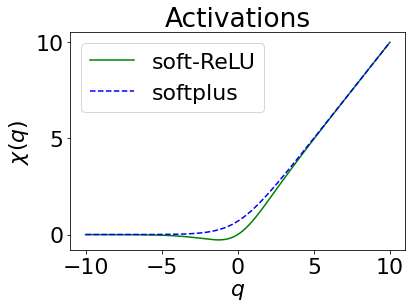
\includegraphics[scale=0.5]{figs/act.png}
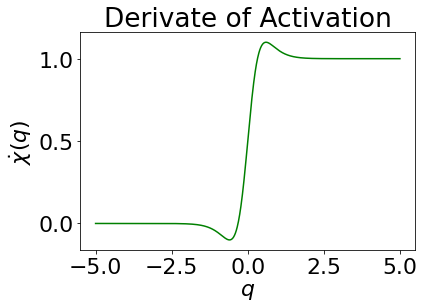
\includegraphics[scale=0.5]{figs/der-act.png}
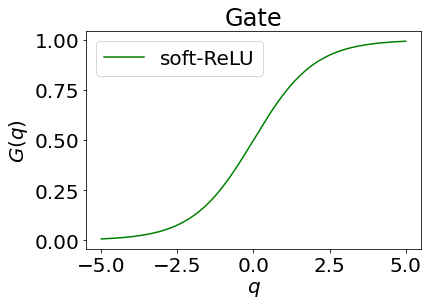
\includegraphics[scale=0.5]{figs/gate.png}
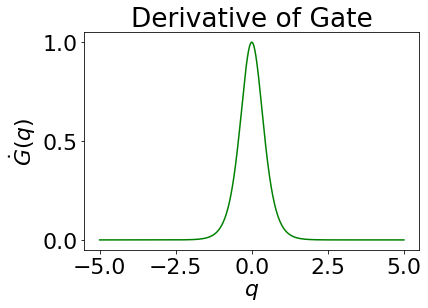
\includegraphics[scale=0.5]{figs/der-gate.png}
%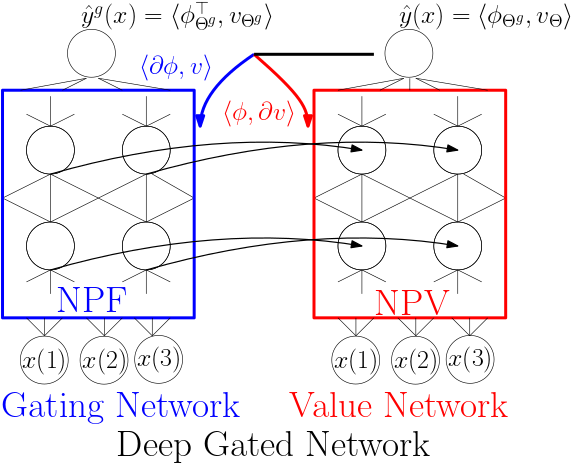
\includegraphics[scale=0.5]{figs/nntwin-blck.png}
%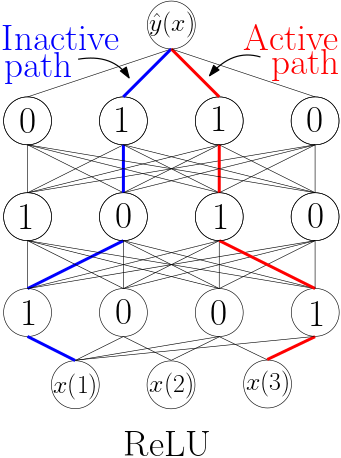
\includegraphics[scale=0.5]{figs/nn.png}
%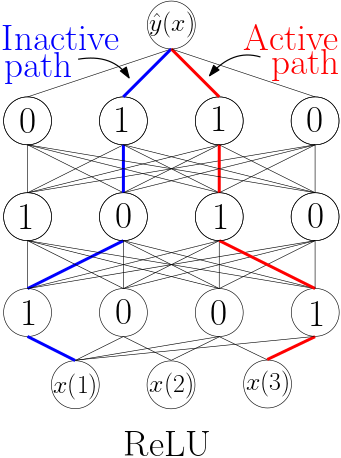
\includegraphics[scale=0.5]{figs/nn.png}
\end{tabular}
}
%\end{minipage}
%\begin{minipage}{0.18\columnwidth}
%\resizebox{\columnwidth}{!}{
%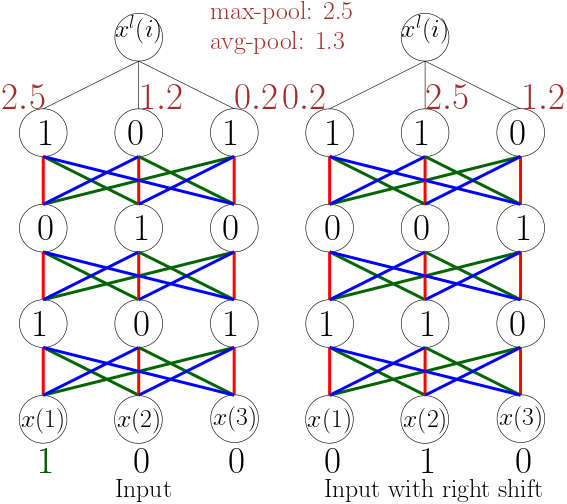
\includegraphics[scale=0.5]{figs/nnconv.png}
%}
%\end{minipage}
\caption{Activations and Gates}
\label{fig:actgate}
\end{figure}

\textbf{Neural Path Kernel} (NPK) matrix is given by $H_{\Theta}=\Phi^\top_{\Theta}\Phi_{\Theta}$, which has a special \emph{Hadamard} structure as given in \Cref{lm:npk} below.
\begin{lemma}[\textbf{Neural Path Kernel (NPK)}]\label{lm:npk}
Let $p\rsa i$ denote the fact that path $p$ passes through input node $i\in[d_{in}]$, and let $\Lambda_{\Theta}(s,s')\stackrel{def}{=}\sum_{p\rsa i} A_{\Theta}(x_s,p) A_{\Theta}(x_{s'},p)$, $\forall s,s'\in[n]$, any $i\in [d_{in}]$. It follows that $H_{\Theta}= \Sigma\odot\Lambda_{\Theta}$, where $\odot$ stands for the Hadamard product, and $\Sigma \in \R^{n\times n}$ is the input Gram matrix.
\end{lemma}
In the \Cref{lm:npk} above, $\Lambda_{\Theta}\in\R^{n\times n}$ is the correlation matrix of the active sub-networks of different input pairs $s,s'\in[n]$. Note that the definition of $\Lambda$ is not dependent on the choice of input node $i$, because, the terms inside the summation depend only on the path followed from the first layer onwards and excludes the input node.
\begin{lemma}\label{lm:nec}
Let $A\in\R^{u\times v}$ and $B\in\R^{w\times u}$, and let $\rho_{\min}(M)$ and $\rho_{\max}(M)$ denote the smallest and the largest eigenvalue of a matrix $M\in\R^{r\times r}$. Then it follows that $\rho_{\min}(A^\top A)\rho_{\max}(B^\top B)\geq \rho_{\min}(A^\top B^\top BA)$.
\end{lemma}
\begin{theorem}[\citet{ando}] 
For two Hermitian matrices $A\in \C^{d\times d}$ and $B\in \C^{d\times d}$, $\lambda_{\min}(A\odot\B)\geq \lambda_{\min} (AB)$. 
\end{theorem}
\begin{lemma}\label{lm:suf}
For two positive definite symmetric matrices $A$ and $B$, $\lambda_{\min}(AB)\geq \lambda_{\min} (A)\lambda_{\min}(B)$. 
\end{lemma}
\textbf{Remarks:}\\
$1.$ From \Cref{lm:nec}, a necessary condition to ensue that $\rho_{\min}(K^v_{\Theta})$ is bounded away from zero is to ensure that $\rho_{\min}(H_{\Theta})$ is bounded away from $0$. \\
$2.$ From \Cref{lm:suf}, a sufficient condition to ensue that $\rho_{\min}(H_{\Theta})$ is bounded away from zero is to ensure that $\rho_{\min}(\Lambda_{\Theta})$ and $\rho_{\min}(\Sigma)$ bounded away from $0$.
\begin{comment}
\begin{proof}
Matrix $AB$ is similar to the matrix $B^{\frac12}ABB^{-\frac12}$. Thus $\lmin{AB}=\lmin{B^{\frac12}AB^{\frac12}}$.
\begin{align*}
\min_{x: \norm{x}^2=1} x^\top B^{\frac12}AB^{\frac12} x &=  \left(\min_{y: y=B^{\frac12} x, x: \norm{x}^2=1 }y^\top A y \right)\\
%&\geq  \left(\min_{y: \norm{y}^2= \min_{x\in \R^d: \norm{x}^2=1} x^\top B x }y^\top A y \right)\\
&\geq \left(\min_{x: \norm{x}^2=1}x^\top B x \right) \left(\min_{y: \norm{y}^2=1 }y^\top A y \right)
\end{align*}
\end{proof}
\end{comment}